%%%% CS 383 HW #5 - hw5-team_lambda.tex
%%%% Due on BBLearn before 10pm on Friday 3/25/2016


%##########################################################################################################################################################################
% Header
%##########################################################################################################################################################################
\documentclass[11pt]{report}

\usepackage{graphicx}
\usepackage{caption}

\marginparwidth 0.5in 
\oddsidemargin 0.25in 
\evensidemargin 0.25in 
\marginparsep 0.25in
\topmargin 0.0in 
\textwidth 6in \textheight 8.5in

\title{Squire: HW5 Individual Contribution}
\author{Kevin Morales (Mora5651) }

\begin{document}

\maketitle

\tableofcontents


%##########################################################################################################################################################################
% Overview
%##########################################################################################################################################################################
\chapter{Overview and Scope}
    \begin{minipage}{1\textwidth}
        \begin{center}
            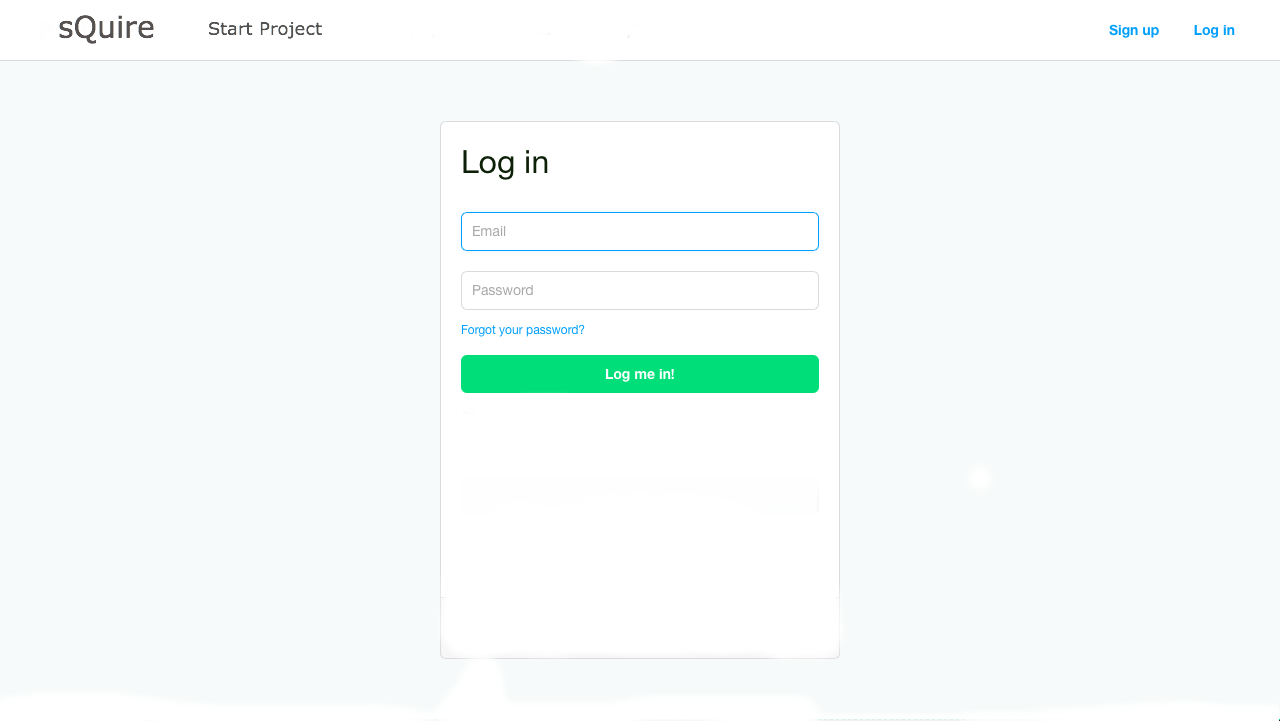
\includegraphics[width=0.7\textwidth]{mockups/mockup-authentication-Login-mora5651}
        \end{center}
        \captionof{figure}{"Squire is a web-based collaborative software development environment with a project development center. Squire will allow multiple users to edit files and communicate in real time. Projects can be ``stubbed'' out by a user and then other users can join and/or vote to support for their favorite projects. After a certain amount of support, planning, and documentation is reached for a project, the project becomes a fully fleged project and then community development can start. Think ``kickstarter for code'' where people pledge their help with the project and not just financial support."}
    \end{minipage}


%##########################################################################################################################################################################
% Statecharts
%##########################################################################################################################################################################
\chapter{State Charts}
    \section{Communication (jank6275)}
    \pagebreak
        \begin{minipage}{1\textwidth}
            \begin{center}
                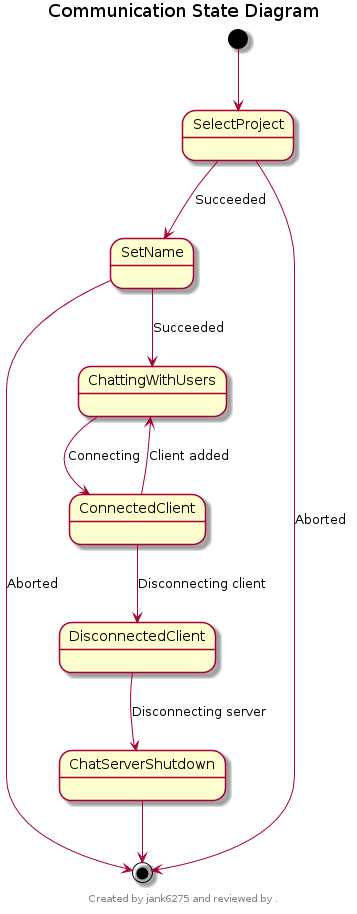
\includegraphics[width=0.5\textwidth]{diagrams/statechart-communication}
            \end{center}
            \captionof{figure}{A statechart that shows the various states of the communication system.}
        \end{minipage}

%##########################################################################################################################################################################
% Mockups
%##########################################################################################################################################################################
\chapter{User Interface Mockups}
    \section{Squire Editor (jank6275)}
    \begin{minipage}{1\textwidth}
        \begin{center}
            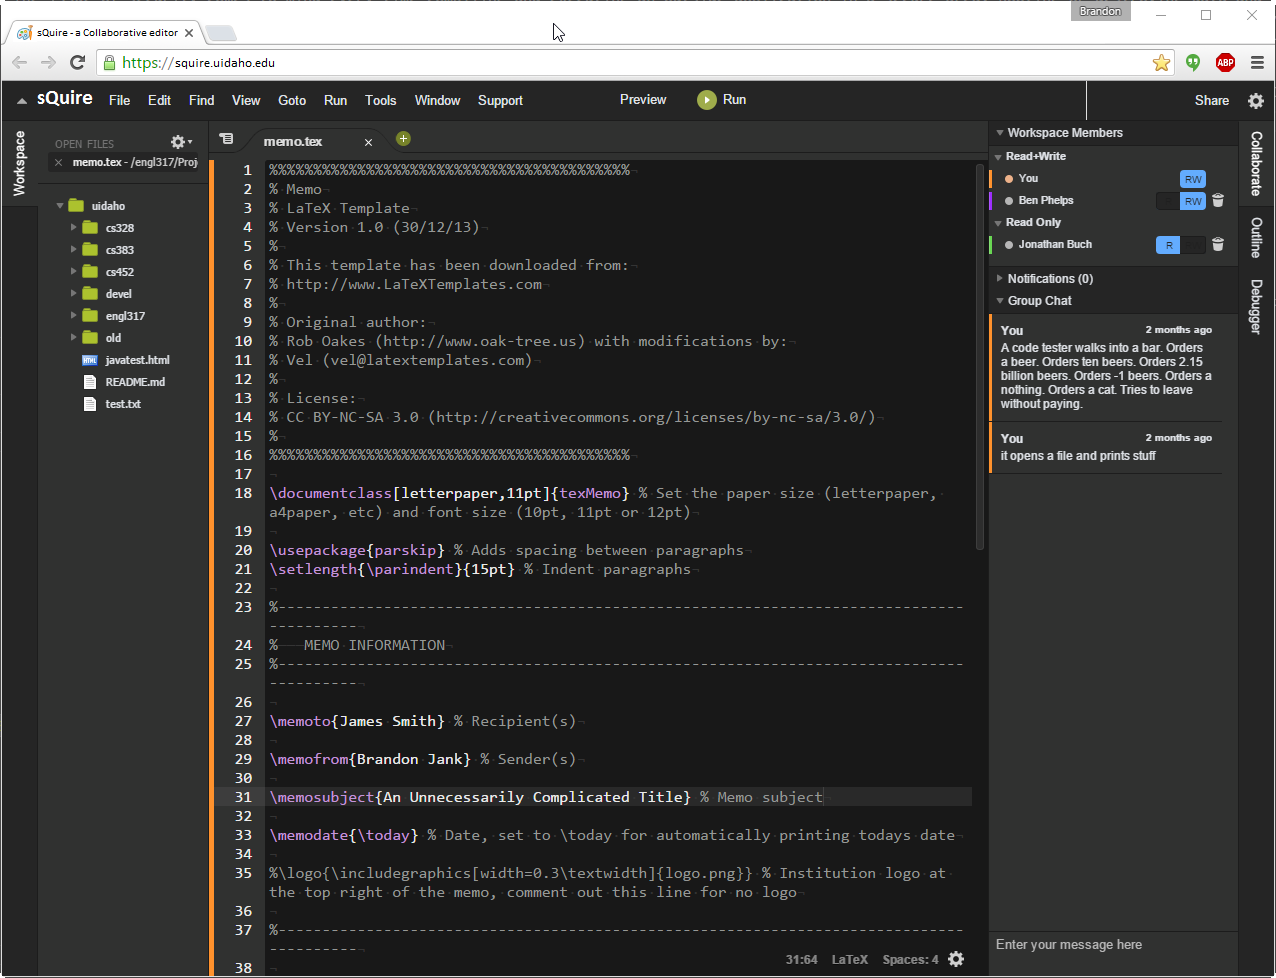
\includegraphics[width=0.9\textwidth]{mockups/mockup-editor-jank6275}
        \end{center}
        \captionof{figure}{What we envision Squire IDE to look like.}
    \end{minipage}
    
    \section{Squire Chat (jank6275)}
    \begin{minipage}{1\textwidth}
        \begin{center}
            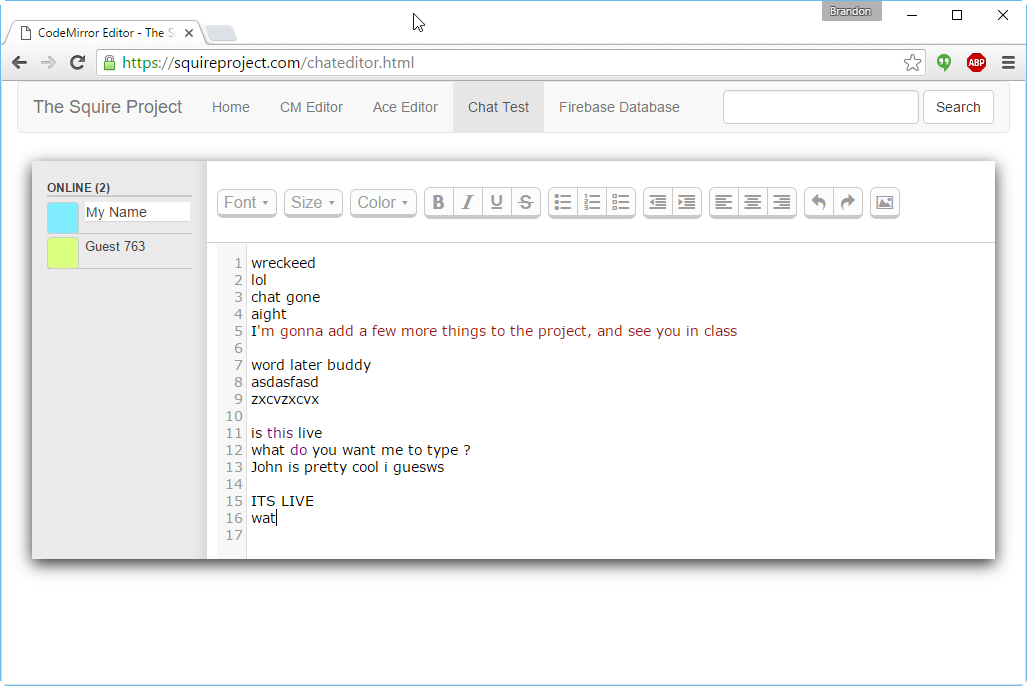
\includegraphics[width=0.9\textwidth]{mockups/mockup-communication-jank6275}
        \end{center}
        \captionof{figure}{How communication could work in squire.}
    \end{minipage}

%##########################################################################################################################################################################
% Prototype Implimentations
%##########################################################################################################################################################################
\chapter{Prototype Implementations}
    \section{Server Stack (jank6275)}
    \begin{minipage}{1\textwidth}
        \begin{center}
            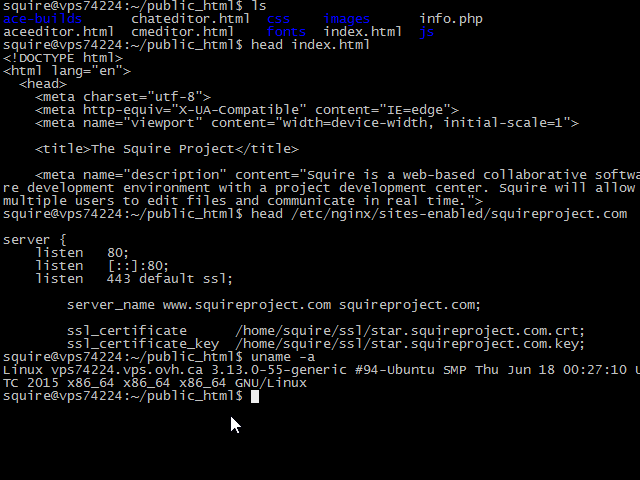
\includegraphics[width=0.9\textwidth]{protos/proto-serverstack-jank6275}
        \end{center}
        \captionof{figure}{The internet domain squireproject.com was registered and an SSL certificate was generated for secure communications. A virtual private server was provisioned and Ubuntu 14.04 installed and then hardened to common network attack vectors. Nginx and MySQL were installed and configured. The web content was written in HTML and bootstrap CSS.}
    \end{minipage}

% EOD
\end{document}